\documentclass{article}


\usepackage{arxiv}

\usepackage[utf8]{inputenc} % allow utf-8 input
\usepackage[T1]{fontenc}    % use 8-bit T1 fonts
\usepackage{hyperref}       % hyperlinks
\usepackage{url}            % simple URL typesetting
\usepackage{booktabs}       % professional-quality tables
\usepackage{amsfonts}       % blackboard math symbols
\usepackage{nicefrac}       % compact symbols for 1/2, etc.
\usepackage{microtype}      % microtypography
\usepackage{lipsum}
\usepackage[dvipsnames]{xcolor}
\usepackage{graphicx}
\graphicspath{ {./images/} }
\usepackage{subcaption}
\usepackage{amsmath}
\usepackage[ruled,vlined]{algorithm2e}
\usepackage{authblk}
\usepackage{float}
\usepackage{subcaption}
\usepackage{booktabs}
\usepackage{listings}
\usepackage{xcolor}

\lstset{
    inputencoding=utf8,
    extendedchars=true,
    literate=
      {“}{{``}}1
      {”}{{''}}1
      {–}{{-}}1
      {—}{{--}}1
      {…}{{...}}1
      {→}{{$\to$}}1
}

\lstdefinestyle{promptstyle}{
    basicstyle=\ttfamily\scriptsize,   % monospaced & very small font
    backgroundcolor=\color{teal!10},    % light gray background
    frame=single,                       % box around listing
    rulecolor=\color{black},            % box colour
    breaklines=true,                    % automatic line wrap
    postbreak=\mbox{\textcolor{red}{$\hookrightarrow$}\space}, % nice wrap marker
    captionpos=b,                       % caption at bottom
    numbers=none,                       % no line numbers
    keepspaces=true                     % respect spacing/indent
}

\lstdefinestyle{baselinestyle}{
    basicstyle=\ttfamily\scriptsize,   % monospaced & very small font
    backgroundcolor=\color{orange!10},    % light gray background
    frame=single,                       % box around listing
    rulecolor=\color{black},            % box colour
    breaklines=true,                    % automatic line wrap
    postbreak=\mbox{\textcolor{red}{$\hookrightarrow$}\space}, % nice wrap marker
    captionpos=b,                       % caption at bottom
    numbers=none,                       % no line numbers
    keepspaces=true                     % respect spacing/indent
}

\title{Leveraging Spreading Activation for Improved Document Retrieval in Knowledge-Graph-Based RAG Systems}


\author[2]{
    Jovan Pavlović
}
\author[1,2, 3]{
    Miklós Krész
}
\author[1,2]{
    László Hajdu
}

\affil[1]{
    \textbf{InnoRenew CoE, UP IAM, University of Primorska}
        }
\affil[2]{\textbf{UP FAMNIT, University of Primorska}}
\affil[3]{\textbf{University of Szeged, Department of Applied Informatics}}


\begin{document}
\maketitle
\begin{abstract}
Despite initial successes and a variety of architectures, retrieval-augmented generation (RAG) systems still struggle to reliably retrieve and connect the multi-step evidence required for complicated reasoning tasks. Most of the standard RAG frameworks regard all retrieved information as equally reliable, overlooking the varying credibility and interconnected nature of large textual corpora. GraphRAG approaches offer potential improvement to RAG systems by using knowledge graphs to capture entity relationships and enable multi-step reasoning, but their impact is often limited by the need for accurate graph representations (often costly to curate or unreliable to induce automatically), as well as by their continued dependence on large language models (LLMs) to navigate the graph and guide evidence selection.  In this paper, we propose SA-RAG framework that uses a spreading activation algorithm to retrieve information from a corpus of documents connected by an automatically constructed heterogeneous knowledge graph. By operating on this heterogeneous structure, the method reduces reliance on semantic knowledge graphs that can be incomplete due to information loss during the graph construction process, while avoiding LLM-guided graph traversal. Experiments show that SA-RAG achieves better or comparable performance than several state-of-the-art methods and can be integrated as a modular component within different iterative pipelines. When combined with chain-of-thought iterative retrieval, it yields up to a 39\% absolute improvement in answer correctness over naive RAG, while achieving these results with small open-weight language models, supporting its use in settings with limited computational resources.
\end{abstract}


% keywords can be removed
%\keywords{First keyword \and Second keyword \and More}


\section{Introduction}
Initially proposed in~\cite{guu2020retrieval, lewis2020retrieval}, Retrieval-Augmented Generation (RAG) has become a popular technique for improving the capabilities of Large Language Models (LLMs) across various tasks, including question answering and code generation.  The basic idea of RAG is to provide LLM access to an external, easily updatable knowledge source by integrating it with the Information Retrieval (IR) component. This technique aims to improve the quality of LLM responses by reducing hallucinations and enhancing text creation accuracy and coherence. Numerous enhancements to the foundational RAG paradigm have been further proposed, ranging from innovative pipeline designs to improvements in individual components. Additionally, several surveys have been conducted to classify, decompose, and identify key elements within the myriad of proposed methodologies, helping track their evolution and highlighting promising future directions~\cite{zhao2024retrieval, fan2024survey, gao2023retrieval, gupta2024comprehensive}. 

A particularly active research area explores the combination of RAG with graph-based systems that represent diversified and relational information. The goal of these integrations is to improve performance on complex tasks involving large, structured, and interconnected knowledge corpora, resulting in methodologies sometimes referred to as GraphRAG. Comprehensive surveys covering the background, components, downstream tasks, and industrial use cases of GraphRAG, as well as the technologies and evaluation methods used, are available in~\cite{peng2024graph, han2024retrieval}. 

As mentioned in~\cite{peng2024graph}, knowledge graph question answering (KGQA) is a key natural language processing task that has motivated the development of KG-based systems aimed at responding to user queries through structured reasoning over predefined knowledge graphs~\cite{zhang2021neural, lavrinovics2025knowledge, pan2024unifying}. The multi-hop question answering (MHQA) task is a related but broader concept, commonly applied in areas such as academic research, customer support, and financial or legal inquiries, where a comprehensive analysis of multiple textual documents is required. In this scenario, given a document corpus, the QA system generates responses to user queries by reasoning across multiple sources, involving sequential reasoning steps where responses at one step may rely on answers from prior steps. Several standard and graph-based RAG methodologies have been proposed to enhance the performance of LLMs on this specific task~\cite{zhang2023end, jeong2024adaptive, wang2024knowledge, jimenez2024hipporag}. Despite significant advancements, most of these approaches still rely primarily on standard or iterative retrieve-read-answer workflows, which are enhanced by optimized pipeline components, LLM decision-making, or LLM-guided graph traversal~\cite{singh2025agentic, fan2024survey}. However, hallucination and weak faithfulness remain unresolved problems in the context of MHQA. LLM-guided iterative retrieval may fail due to myopic knowledge exploration, retrieving context based on partial reasoning from previous steps, which can be incorrect or contain fabricated information. Similarly, one-step RAG systems with optimized retrieval components may fetch more useful evidence in the retrieved context, but they often introduce a lot of noise or fail to capture information from "bridge" documents whose entities or phrases are not mentioned in the input query. Thus, although adding improvements to vanilla RAG, the paradigm behind these advanced methods stays fundamentally the same, thereby overlooking powerful and well-established IR algorithms that can automatically identify relationships between documents and adapt retrieval for multi-hop query scenarios.

Motivated by this gap, this paper proposes a novel GraphRAG framework that integrates Spreading Activation (SA), a search method for associative networks originally developed in cognitive psychology. Beyond information retrieval~\cite{crestani1997application}, SA has been successfully applied in several domains, including natural language processing~\cite{pollack1982natural, tsatsaronis2007word}, robotics, and reinforcement learning~\cite{kono2019activation}. Specifically, we propose a RAG system that operates on a hybrid structure combining a knowledge graph with textual information from knowledge documents. It retrieves relevant documents from textual corpora by executing an SA algorithm through the knowledge graph, identifying and fetching chunks of text with the most pertinent information required to answer the multi-hop query, thereby capturing the reasoning structure and key relationships between entities mentioned in the query. 

To the best of our knowledge, only one prior paper has integrated RAG and SA-based methodologies~\cite{wu2025kg}. However, our approach differs in several key respects. First, the mentioned system relies on human-crafted knowledge graphs, whereas our pipeline includes an automated knowledge-graph construction phase. Second, it uses a prompted LLM to perform the SA procedure and expand the initially retrieved subgraph; by contrast, we perform SA automatically by exploring the knowledge graph in a breadth-first manner and spreading the activation based on edge weights assigned by an embedding model. Finally, the prior method fine-tunes the LLM to improve its instruction-following abilities, while our method requires no retraining. Overall, we believe our methodology provides an innovative direction for enhancing retrieval-augmented generation by leveraging a cognitively inspired mechanism that emphasizes associative relevance rather than surface-level similarity.

We summarize the key contributions of our work as follows:

\begin{enumerate}
    \item We introduce a knowledge-base indexing strategy that uses a prompt-tuned LLM to construct text-attributed knowledge graphs, linking documents and enabling the use of graph-traversal techniques during document retrieval.
    \item We introduce a novel integration of the Spreading Activation algorithm with LLMs, aiming to enhance grounded reasoning over large corpora of interconnected textual documents.
    \item We demonstrate notable performance improvements of our pipeline over standard RAG frameworks through experiments on two well-known multi-hop QA benchmarks. The results show that our SA-based document retrieval method enables more efficient exploration of the knowledge corpus than dense-vector retrieval alone, going beyond mere semantic similarity and enabling LLMs to produce more accurate answers to complex multi-hop questions.
    \item When combined with iterative retrieval, our method yields absolute improvements in answer accuracy ranging from 25\% to 39\% relative to naive RAG.
    \item Given the fact that our experiments are performed with small-open weight models, which require less computational power, and yet we achieved significant results, we highlight the potential for deploying high-performance reasoning systems in resource-constrained environments.
\end{enumerate}

The rest of this paper is organized as follows. Section 2 reviews the background and related work. Section 3 presents the motivation behind the proposed SA-RAG method alongside its implementation details. Sections 4 and 5 describe the experimental setup and results, respectively. Finally, Section 6 concludes the paper by discussing limitations and future directions. The code used to run the experiments is available at \url{https://github.com/jomibg/sa-rag}

\section{Background and Related Work}

This section reviews the main lines of research that the proposed method builds on. We begin by discussing how RAG has evolved to support multi-hop reasoning; We then outline how GraphRAG systems use graph structure to guide retrieval and generation. Finally, we introduce spreading activation and explain how its controlled variants can uncover "bridge" evidence that standard similarity searches miss.

\subsection{RAG and Multi-Hop Question Answering}
Although traditional RAG systems enhance LLM capabilities across both standard and knowledge-intensive NLP tasks, they encounter several critical limitations when handling complex reasoning. This is particularly evident in MHQA~\cite{mavi2024multi}, where the system is required to reason across multiple pieces of information or documents to answer complicated questions. Traditional systems rely on simple, single-shot retrieval, which often fails to capture all necessary information or may even overload the LLM’s context window with unnecessary or incorrect data. Numerous additions are proposed through the evolution of RAG paradigms with the aim of overcoming naive  "retrieve-then-generate" methodology, which, according to the survey~\cite{fan2024survey}, can be classified into two categories: \textit{training-free} and \textit{training-based} approaches. Training-free approaches aim to optimize RAG pipelines through techniques such as prompt engineering, in-context learning, improved organization of data in the knowledge corpus, or agentic design~\cite{singh2025agentic}. In contrast, training-based methods rely on fine-tuning the retriever and generator components to boost the system’s performance on downstream tasks.

Since our methodology does not require pre-training of any RAG components, we highlight a few training-free approaches that have been shown to enhance the performance of RAG systems in multi-hop question answering.

Multiple advanced RAG techniques use \textit{query expansion} as a means to improve retrieval steps by generating richer, semantically varied reformulations of the original question to match more relevant evidence from the knowledge corpus.

Articles~\cite{wang2023query2doc, gao2023precise} propose methods that first generate plausible answer-like passages for the input query and then embed them using sparse or dense encoders to match semantically similar real documents from the knowledge base.

Papers~\cite{ma2023query, fu2021decomposing} suggest that complex, implicit, or multi-hop queries should be rewritten, disambiguated, or decomposed before retrieval to optimize the fetched context.

Several papers have discussed the implementation of iterative retrieval procedures to enhance system performance on multi-hop questions, suggesting that retrieval should be viewed as an operation interleaved with the LLM’s own intermediate reasoning.

In~\cite{trivedi2022interleaving} authors propose a RAG system integrated with Chain‑of‑thought (CoT), a prompting technique, where each CoT step becomes the query for the next retrieval. Similarly, ~\cite{kim2023tree} proposes system based on Tree‑of‑Thoughts (ToT) structured prompting framework; starting from an underspecified root question, the model generates candidate clarification subquestions, prunes uninformative branches, and for each surviving node runs a retrieval round targeted to that clarification, so that by the time the leaves are answered the system has accumulated disjoint, high-precision evidence for answering the original query.

Few papers propose integrating advanced RAG mechanisms with reflection modules that allow LLMs to determine the most suitable retrieval strategy based on the input query~\cite{jeong2024adaptive, wang2023self, asai2024self, crag}. By reflecting on the question, the LLM can choose whether to perform simple retrieval, engage in iterative retrieval steps, or rely on its own internal knowledge. Some systems can dynamically guide the direction and number of retrieval steps, evaluate the relevance of retrieved content~\cite{asai2024self}, or make use of external tools such as online search~\cite{crag}.

Many of these training-free methods are plug-and-play, agnostic to the specific retriever or model, and can be combined both with each other and with different RAG paradigms or fine-tuned models.

\subsection{GraphRAG}
The GraphRAG paradigm~\cite{peng2024graph, han2024retrieval} aims to extend RAG systems by leveraging the structured relationships and hierarchical organization of information in graph data to improve multi-hop reasoning and contextual understanding.

One of the first successful GraphRAG systems, introduced in~\cite{edge2024local}, was designed for Query-Focused Summarization (QFS), where, provided a query and a document corpus, the system seeks to compress the contents of multiple documents, gathering the identified themes and providing a unified summary of the entire document corpus. The proposed approach focuses on the connection between the summarization task and the inherent modularity of graphs, which allows partitioning of graphs into communities. LLM is first instructed to create a knowledge graph from source texts by extracting entities and relationships between them. The system then uses the Leiden community detection algorithm to partition this graph into hierarchical communities. Finally, each community is summarized separately, and the summaries are combined to produce a final, comprehensive response to the user's question.

With respect to MHQA, few works have received significant attention for effectively integrating graph-based retrieval and reasoning within the RAG. 

LightRAG proposed in~\cite{guo2024lightrag} firstly builds a lightweight knowledge graph over a document corpus by using an LLM to extract entities and relations from chunks. For each node and edge, it then constructs a key–value entry, where the key is a short textual label and the value is a concise summary derived from the source documents. At query time, another language model analyses the input and produces two sets of query terms, one focusing on concrete objects and relations, and another capturing broader topics. Terms from the first set are embedded and used for vector search over keys tied to entity nodes, while the broader theme terms are used to match keys associated with relation edges. The retrieved graph elements are expanded by one hop to include their neighbors, then the corresponding value texts are combined into a compact context that is passed to a generative model to produce the final answer.

In~\cite{g-retriever}, the authors present G-Retriever, a framework that leverages the integration of graph neural networks and LLMs. The system efficiently responds to user queries by retrieving relevant subgraphs using a Prize-Collecting Steiner Tree algorithm and translating graph data to a textual representation. The graph encoder and projection layer, which are in charge of aligning subgraph information with the language model's hidden space, are fine-tuned via backpropagation based on the difference between the generated answer and the ground truth. This technique is evaluated on different tasks, ranging from commonsense reasoning and scene comprehension to knowledge-based question answering.

These systems differ, however, from our approach in that they search a constructed knowledge graph to gather relational knowledge, then convert this context into textual form before passing it to the LLM. In contrast, our methodology uses knowledge graph search to match textual documents directly without requiring an intermediate step of transforming graph data into text. 

Another MHQA pipeline is presented in~\cite{jimenez2024hipporag, gutierrez2025rag}. Their proposed approach, HippoRAG, creates a schemaless knowledge graph with instruction-tuned LLM. When a query is received, the language model extracts the key named entities from the query, which are then mapped to their associated nodes in the knowledge graph using similarity scores calculated by the retrieval encoder. These nodes serve as seeds for a graph search using the Personalized PageRank algorithm, which propagates activation through the network to identify nodes that may be associated with the provided question. Since this approach is similar to our solution in its use of a knowledge graph to retrieve relevant textual passages, we adopt it as a natural baseline in our experiments.

\subsection{Spreading Activation}
Paper~\cite{quillian1967word} proposed that human semantic memory is organized as a network and was one of the first to implement a semantic network model of knowledge in a computer. In this framework, concepts and their properties were modeled as nodes in a network connected by links encoding semantic relationships, arranged hierarchically so that more specific concepts point to more general ones. Activation spreading was introduced as a mechanism to search this network in order to verify factual sentences (e.g., canary is a bird). This was achieved by activating a concept and letting that activation move through the network until it intersected with activation from another concept. Later in \cite{collins1969retrieval} the computational model was tested against human performance in sentence–verification tasks, where people’s response times to statements at different hierarchical levels (e.g. “a canary is a bird” vs. “a canary is an animal”) were compared to the model’s predictions, showing that longer network traversals correlate with slower verification times. This model was then modified in~\cite{collins1975spreading, anderson1983spreading} to account for varying association strengths and decay of activation over distance, dropping the requirement that the network is strictly hierarchical. The spreading mechanism was generalized so that activation spreads from a currently active concept to all linked concepts, in parallel, with the strength that depends on link weight and fades with distance.

After its development in the field of cognitive psychology, SA was adapted in later works as a computational tool for information retrieval and recommender systems. In this context, original principles were repurposed so that input queries or user profiles trigger activation in a graph of terms, documents, or items, and the resulting activation pattern is used to rank candidates by their inferred relevance or interest.

In~\cite{salton1988use}, the authors argued that SA can be implemented in IR systems to overcome the limitations of standard TF-IDF-based approaches, particularly when the user’s wording does not match the wording of the documents and when relevant documents are only indirectly connected to the query. They proposed a system using network representation of the document corpus, where both documents and index terms are modeled as nodes, interconnected by various types of links: term–document links modeling the presence of a term in a document, term–term links connecting terms that frequently co-occur or are semantically related according to a thesaurus, and document–document links connecting documents that share co-occurring terms. In this setting, the SA procedure starts by taking the query terms or documents retrieved by the normal vector-space search and assigning them an initial activation value. The activation then propagates from every active node to its neighbors, with the amount passed along each link scaled by the link’s strength, and nodes whose accumulated activation exceeds a specified threshold are finally retrieved. However, the authors implemented and evaluated only a simplified version of the described procedure due to the computational costs of a full implementation at that time. They concluded that the spreading activation procedure is a useful complementary module to standard IR systems, but it needs to be constrained by limiting the number of steps to just a few hops from the original query nodes and by using a decay factor smaller than one. Later works expanded criticism of unconstrained SA along the same lines; In~\cite{berthold2009pure}, the authors showed that the pure SA algorithm, where activation propagates over all outgoing links with no limits on hops, fan-out, or thresholds, converges to a fixed state and retrieval results become nearly independent of the input query. This underscores that heuristic constraints in applied SA-based systems are not just pragmatic features but essential for the retrieval of query‐dependent results.

More recent applications in IR and recommendation systems, therefore, employ adapted, task-driven variants of SA, where the spread is guided by the user’s information need or context and then combined with conventional ranking steps. In~\cite{ngo2014discovering}, the authors propose a semantic text search method based on SA, which, given an input query, performs named entity recognition and relationship extraction, then maps the extracted elements to an ontology to represent the query as a concise structured pattern. The method then spreads activation only to concepts that match the relationships actually expressed in the query, as well as to closely related information such as alternative names or parent categories. Activated concepts are retrieved and appended to the original query to form an expanded query, which is then executed by a classical sparse-vector search engine, allowing ordinary document ranking to exploit both the user’s words and the newly discovered latent concepts.

Article~\cite{blanco2010adapting} describes a semantic, knowledge-based recommender built around an ontology that stores domain concepts, user interests, and item descriptors, and then runs a controlled spreading of activation from the user profile toward semantically adjacent items so that recommendations reflect both explicit preferences and latent relations present in the knowledge base. The system routes the activation only through specific, typed links in the ontology, assigning weight to each link based on its type and finally ranking associated items according to their activation values and standard recommendation filters. Similarly, \cite{papneja2018context} extends ontology-based SA with contextual cues, such as current task or situational attributes, so that activation is fired not only from the long-term user profile but also from context nodes. Activation propagates only along meaningful ontology links, with decay and link weights, thereby avoiding uncontrolled diffusion through the network.

\section{Methodology}
In this section, we formalize the retrieval task and objective. We begin with a motivational example in which we explain the main advantages of using spreading activation for semantic search on knowledge graphs in the presence of multi-hop questions. We then walk through the complete SA-RAG pipeline. Each component is explained in turn, from indexing and subgraph construction to the exact details of the information retrieval method, and finally, the answer generation. We also cover key parameters and design choices that shape the behavior of the system

\subsection{Motivation}
Consider an IR system posed with the question \textbf{"What is the capital of the county that shares a border with the county that contains the birthplace of Erik Jensen?"} (query \textit{4hop1\_\_707078\_378185\_282674\_759393} from the MuSiQuE dataset). Assume the system's knowledge base can be represented as a weighted knowledge graph displayed in Figure~\ref{fig:kg_cs}, where the weights on edges represent semantic similarity between the query and the relationships that these edges encode, and imagine that each entity is associated with a textual description. In order to provide the context necessary for answering the question, the system must gather information about five entities lying along the shortest path from the node \textit{"Erik Jensen"} to the node \textit{Green Bay, Wisconsin} (the so-called \textit{golden} entities). Of course, the trivial solution would be to select all the entities and reason through all of the textual descriptions; however, this would introduce a lot of irrelevant information into the deduction procedure. Moreover, if the working memory of the reasoning agent (which is the context window in the case of LLMs) is limited, it would be necessary to filter out some of the nodes.

\begin{figure}[t]
  \centering
  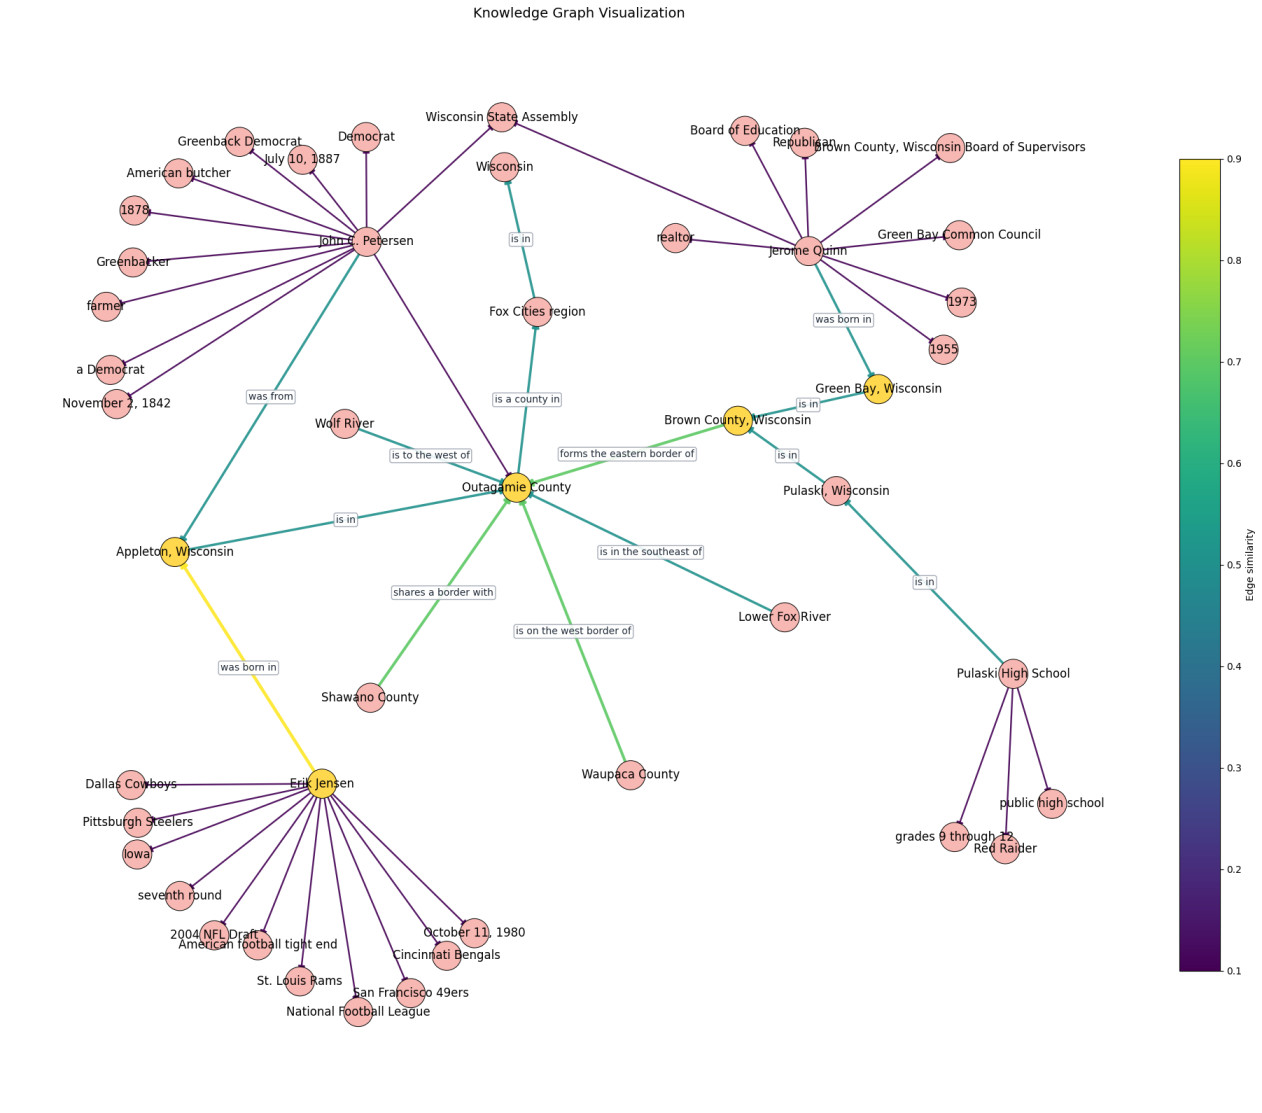
\includegraphics[width=0.8\linewidth]{kg.jpg}
  \caption{A knowledge graph representing the system's knowledge base for
the example query. Edge weights reflect the semantic similarity between the input question and the relationships encoded by each edge. Yellow nodes represent \textit{golden} entities holding information necessary for answering the query}
  \label{fig:kg_cs}
\end{figure}

Now suppose that we can collect at most 10 entities and that the text search algorithm identifies the descriptions of nodes \textit{"Erik Jensen"} and \textit{"Outagamie County"} as the semantically most similar to the input question. Also, let the edge weights $w_e$ be calculated by the following simple rule:
\begin{itemize}
    \item If the corresponding relationship expresses location and contains the word "border" or "born", let $w_e := 0.7$
    \item If the relationship expresses location (such as "is in"), let $w_e := 0.5$
    \item Otherwise, let $w_e:=0.1$
\end{itemize}

Of course, more nuanced edge weights can be derived by comparing latent representations of questions and entities, produced by state-of-the-art embedding models, but this simplified scheme is sufficient to illustrate the core idea. 

Now, if we want to collect the rest of the relevant entities, we would intuitively look for entities located \textit{"close"} to the initial ones, or nodes that act as bridges \textit{"between"} the known pieces of information. Equivalent intuition leads to the concept of node centrality in network science, which are numbers or rankings meant to summarize a node's position and topological role within the complex network.

Different definitions of centralities have been proposed in the literature~\cite{centrality_zoo}, each designed to capture a different aspect of a node's importance, and several existing GraphRAG frameworks have incorporated such measures into their retrieval pipelines. Notably, the authors of HippoRAG~\cite{jimenez2024hipporag} proposed the usage of Personalized PageRank (PPR) score as a robust metric summarizing the relevance of nodes in the knowledge graph based on specific clues in the input query. Closeness centrality, defined as the reciprocal of the sum of the shortest path distances from a given node to a set of other nodes, provides a complementary, distance-based perspective on node importance. However, we argue that that the SA algorithm subsumes both of these perspectives, providing relevance scores summarizing the intuitive notions of \textit{"closeness"} and \textit{"betweenness"}.

Table~\ref{tab:entity_scores} displays node rankings and associated relevance scores calculated based on PPR, closeness centrality, and the SA algorithm detailed in Algorithm~4. As can be seen, in our example only SA collects all of the \textit{golden} entities associated with our input query. Similarly, Figure~\ref{fig:scores} shows our knowledge graph where the size and color of nodes indicate the relevance scores assigned by each method. It is worth noting, however, that SA exhibits a tendency to assign high relevance scores to non-golden entities, raising the risk of false positives. As elaborated later in this section, we address this limitation through a set of additional mechanisms and hyperparameter choices, seeking to reduce the mentioned negative effects.


\begin{table}[ht]
\centering
\caption{Comparison of entities based on Closeness centrality, PPR score, and SA score.}
\label{tab:entity_scores}
\resizebox{\textwidth}{!}{% <-- Forces everything to fit the exact page width
\begin{tabular}{lclclc}
\toprule
\multicolumn{2}{c}{\textbf{Closeness centrality}} & \multicolumn{2}{c}{\textbf{PPR score}} & \multicolumn{2}{c}{\textbf{SA score}} \\
\cmidrule(r){1-2} \cmidrule(lr){3-4} \cmidrule(l){5-6}
\textbf{Entity} & \textbf{score} & \textbf{Entity} & \textbf{score} & \textbf{Entity} & \textbf{score} \\
\midrule
\textbf{Erik Jensen} & 1.000000 & \textbf{Outagamie County} & 1.000000 & \textbf{Erik Jensen} & 1.0000 \\
\textbf{Outagamie County} & 1.000000 & \textbf{Erik Jensen} & 0.871173 & \textbf{Outagamie County} & 1.0000 \\
\textbf{Appleton, Wisconsin} & 1.000000 & \textbf{Appleton, Wisconsin} & 0.494452 & Shawano County & 1.0000 \\
Shawano County & 0.431818 & John C. Petersen & 0.229822 & Waupaca County & 1.0000 \\
Waupaca County & 0.431818 & \textbf{Brown County, Wisconsin} & 0.199652 & \textbf{Brown County, Wisconsin} & 1.0000 \\
\textbf{Brown County, Wisconsin} & 0.431818 & Fox Cities region & 0.155080 & \textbf{Appleton, Wisconsin} & 1.0000 \\
John C. Petersen & 0.318182 & Shawano County & 0.138262 & John C. Petersen & 1.0000 \\
Wolf River & 0.289773 & Waupaca County & 0.138262 & Fox Cities region & 1.0000 \\
Lower Fox River & 0.289773 & Wolf River & 0.097627 & Pulaski, Wisconsin & 0.9403 \\
Fox Cities region & 0.289773 & Lower Fox River & 0.097627 & \textbf{Green Bay, Wisconsin} & 0.8979 \\
\bottomrule
\end{tabular}%
}
\end{table}

\begin{figure}[ht]
  \centering
  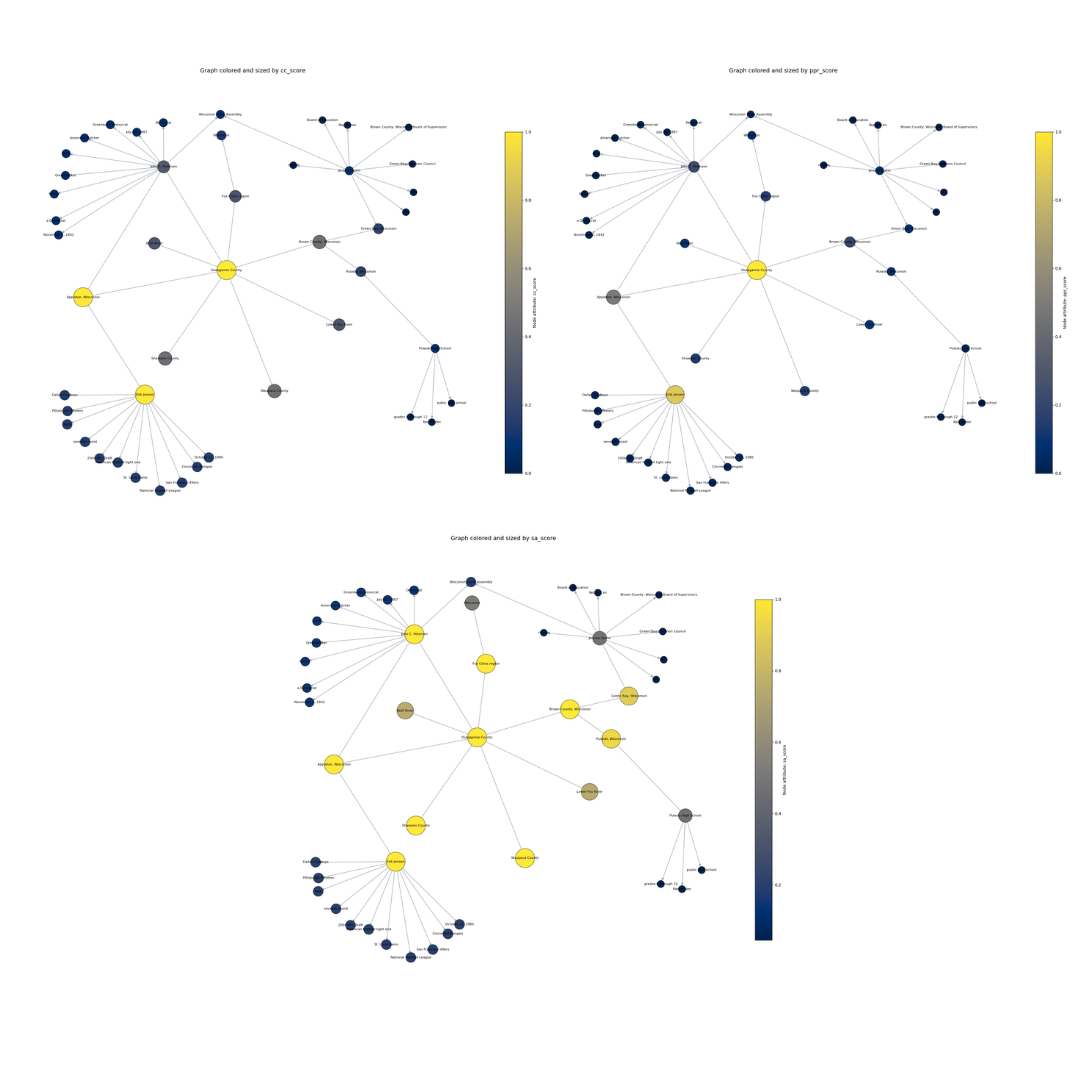
\includegraphics[width=0.8\linewidth]{scores.png}
  \caption{Visual comparison of (normalized) relevance scores assigned to knowledge graph nodes by three retrieval methods: closeness centrality, Personalized PageRank (PPR) and the SA algorithm. Node size and color intensity both scale with the relevance score assigned by each method, larger and brighter nodes are ranked more relevant.}
  \label{fig:scores}
\end{figure}

\newpage
\subsection{Problem definition}
Given a question $q$ and a knowledge base $KB = \{D_1, \ldots, D_n\}$ containing a corpus of textual documents organized in some manner, the system generates an answer $a$ by retrieving a subset of relevant documents $\mathcal{D} \subseteq KB$. Formally, this can be expressed as:  
\begin{align*}
    \mathcal{D} &= R(q, KB) \\
    a &= \text{LLM}(q, \mathcal{D})
\end{align*}
where $R$ denotes the retrieval component of the system, and \textit{LLM} refers to the large language model responsible for generating the answer.  
The objective is to maximize the probability of producing the correct answer $a^*$, that is,  
\[
p(a^* = a \mid q, KB) = \sum_{\mathcal{D} \subseteq KB} p(a^* = a \mid q, \mathcal{D}) \, p(\mathcal{D} \mid q, KB).
\]
Since the generation process is not directly optimized, the task reduces to identifying the subset of documents $\mathcal{D}^*$ that maximizes the probability of providing the correct answer:
\[
\mathcal{D}^* = \arg\max_{\mathcal{D} \subseteq KB} p(a^* \mid q, \mathcal{D}) \, p(\mathcal{D} \mid q, KB).
\]
\subsection{System description}
We summarize the architecture of our RAG system enhanced with a spreading activation–based retrieval mechanism.  It consists of four main stages: indexing, subgraph fetching, spreading activation and document retrieval, and finally, answer generation. These stages are summarized below:
\begin{enumerate}
    \item \textit{Indexing}: In this phase, we break knowledge documents into chunks, create vector embeddings for these text chunks, and use them to build a knowledge graph of the entities, entity descriptions, and relationships mentioned. We also record references between each chunk and every entity it contains by storing the chunks as nodes in the graph, with outgoing links connecting them to the corresponding entity nodes.
    \item \textit{Subgraph fetching}: Given a query, we fetch a subgraph consisting of the most relevant nodes and relations based on the cosine similarity calculated between the vector embedding of the query and the embeddings of entity descriptions. Here, we also determine the set of initially activated entities according to their relevance as indicated by cosine similarity.
    \item \textit{Spreading activation and document retrieval}: We run spreading activation from the initially activated entities to obtain a subset of relevant nodes and fetch the textual paragraphs that mention these nodes. We also record the most relevant relations and combine their textual descriptions with the fetched documents.
    \item \textit{Answer generation}: The LLM then generates a grounded answer using the information from the fetched context.
\end{enumerate}

Figure~\ref{fig:fig1} provides a high-level overview of the proposed methodology. The prompts used at each step of our pipeline are detailed in Appendix B.

\begin{figure}[ht]
  \centering
  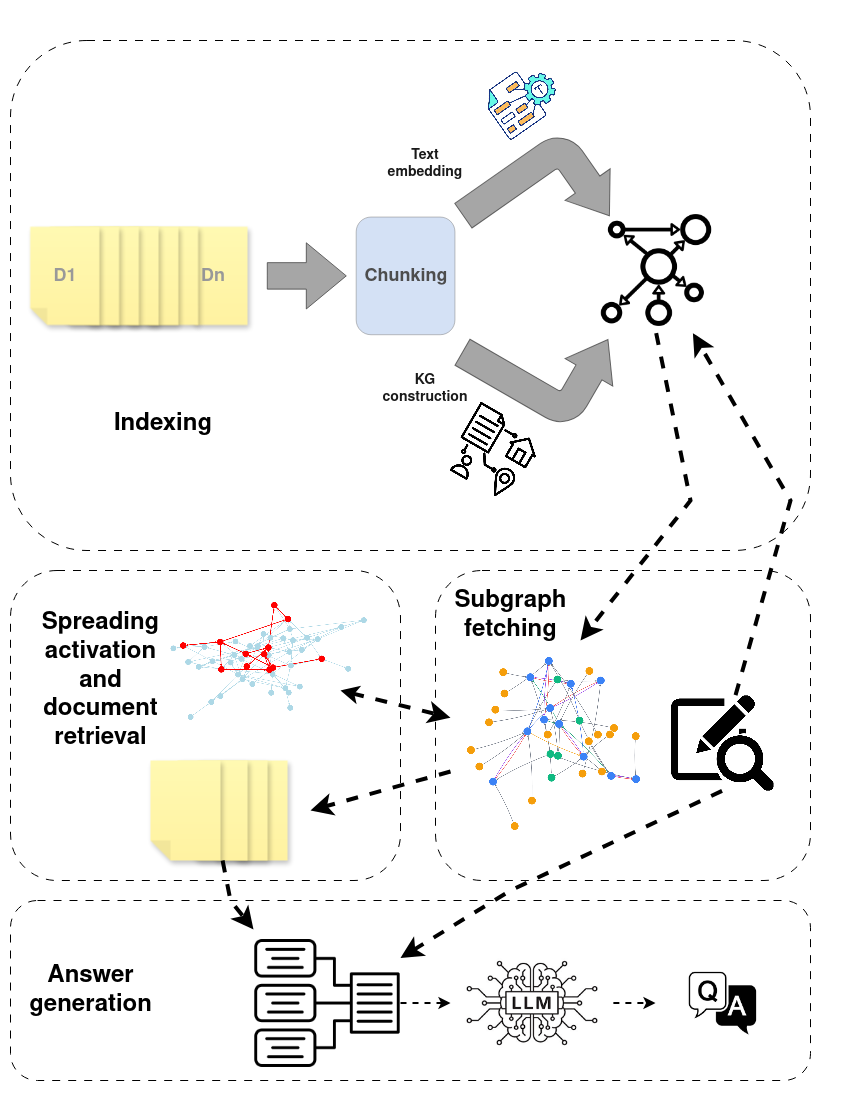
\includegraphics[width=0.5\linewidth]{diagram.png}
  \caption{High-level overview of methodology}
  \label{fig:fig1}
\end{figure}


\subsection{Indexing}
We begin the indexing phase by performing word-based chunking, by splitting input documents into chunks of 500 words with an overlap of 200 words between consecutive chunks. Each chunk is passed to the embedding model and then to a prompt-tuned LLM, which is instructed to extract entities, relations, and entity descriptions from the text. We construct a knowledge graph containing three types of nodes: entities, entity descriptions, and documents  (which represent the textual chunks). The graph also includes three types of links: \textit{describes} and \textit{related\_to}. The \textit{describes} links connect document and entity description nodes to their corresponding entities, while the \textit{related\_to} links connect two entities that are described as related within the text chunk. Additionally, each \textit{related\_to} link stores a string attribute holding the textual description of the relationship between the endpoint entities. Each entity node stores its \textit{name} as well as a list of alternative names within an \textit{aliases} attribute. When adding new elements to the knowledge graph, we ensure that duplicate entities are not created by first checking whether the \textit{name} or any of the \textit{aliases} of the newly extracted entities overlap with those of previously extracted entities.  If the entity already exists, we create new entity description nodes and a \textit{describes} link connecting them to the corresponding entity. Additionally, we create vector embeddings for both entity description nodes and \textit{related\_to} links using the same embedding model applied to the textual chunks. The indexing process is illustrated in Figure~\ref{fig:fig2}.

\begin{figure}[ht]
  \centering
  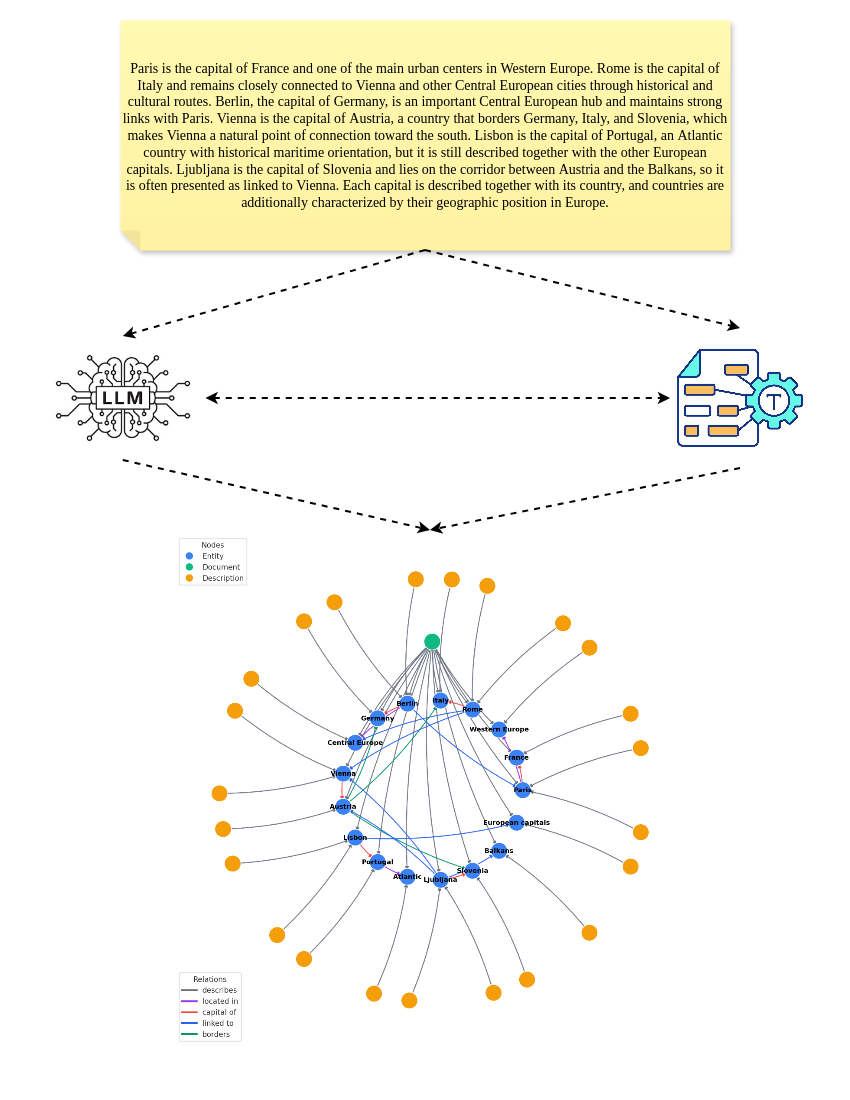
\includegraphics[width=0.7\linewidth]{indexing.png}
  \caption{Knowledge graph creation during the indexing phase. The figure shows an example graph constructed from a single document describing the capital cities of European states. The document node is marked in green, entity description nodes are colored orange, and entity nodes are shown in blue.}
  \label{fig:fig2}
\end{figure}


\subsection{Subgraph fetching}
At this stage, we retrieve the subgraph consisting of entities and relations that are potentially relevant to answering the input query. Specifically, we first identify the top-$k$ entity descriptions whose embeddings have the highest cosine similarity to the query embedding. We then include the entities referenced by these descriptions through incoming \textit{describes} links and expand the graph by retrieving all entities and \textit{related\_to} links within their $n$-hop neighborhood. The “seed” entities matched in the first step are marked as initially activated for the spreading activation process, and each link is assigned a weight equal to the cosine similarity between the query and the link embedding. We set the values of $k$ and $n$ to 3 and 4, respectively, for the MuSiQue experiments, and to 10 and 3 for the 2WikiMultiHopQA experiments, as these parameter choices yielded the best results. The process is illustrated in Figure~\ref{fig:fig3}.

\begin{figure}[ht!]
  \centering
  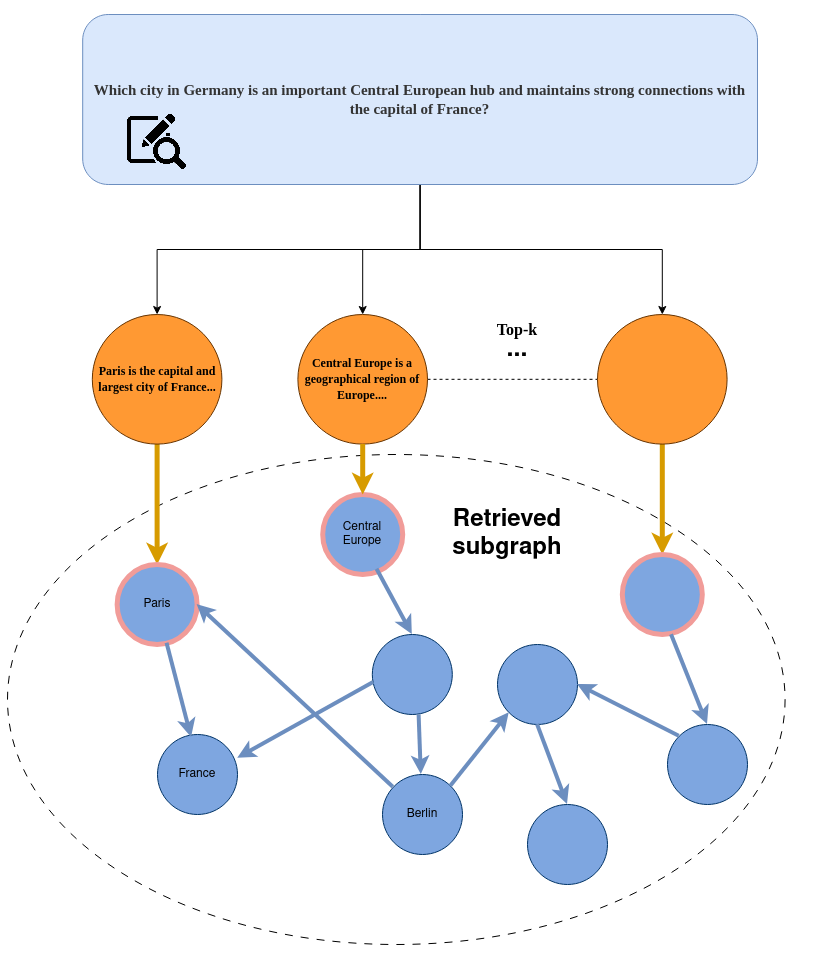
\includegraphics[width=0.7\linewidth]{subgraph.png}
  \caption{Subgraph fetching step: Orange nodes represent the \textit{top-k} entity description nodes, while entity nodes are shown in blue. Links of the \textit{describes} type are colored orange, whereas blue links represent \textit{related\_to} relations connecting entity nodes. Initially activated “seed” entities are indicated by a red border.}
  \label{fig:fig3}
\end{figure}

\newpage
\subsection{Spreading activation and document retrieval}
This stage simulates spreading activation on the retrieved subgraph, starting from the initially activated nodes identified in the previous step. Before the propagation begins, we rescale the edge weights by a linear factor $c$, using the formula $w' = \frac{w-c}{1-c}$. This adjustment helps prevent overactivation, which could otherwise result in nearly every node becoming strongly activated and ultimately leading to context explosion. By experimenting on multiple small samples of approximately 10 questions, we found that setting $c=0.4$ provided the best results in terms of the recall/precision tradeoff. A more detailed illustration of how the value of $c$ impacts the outcome of the spreading activation can be found in Figure~\ref{fig:fig5}.

The SA process operates as follows: initially, activated nodes are assigned an activation value of $a_i = 1$, while all other nodes get a value of $a_j = 0$. Activation then propagates outward from these initially activated nodes to their neighboring nodes in a BFS manner, through the weighted links $w_{ij}$. In each iteration, the activation value of each target node is updated as $a_j = min(a_j + \sum_{i \in N(j)}a_i\cdot w_{ij})$ and after the process is complete, nodes whose activation exceeds the threshold $\tau_a$ are marked as activated. The entire procedure is summarized in Algorithm~\ref{alg:diffusion_process}, and Figure~\ref{fig:fig4} provides a visualization of the SA run on the subgraph retrieved for a multi-hop query from the MuSiQue benchmark.

\begin{algorithm}[ht!]
\caption{Spreading Activation algorithm on entity subgraph}
\label{alg:diffusion_process}
\DontPrintSemicolon

\KwIn{
  Adjacency dictionary $adj\_dict$ mapping entities to outgoing weighted arcs;\\
  Set of initially activated entities $I_a$;\\
  Activation threshold $\tau_{\text{a}}$;
}
\KwOut{
  Set of activated entities $R_a$.
}

\BlankLine

\ForEach{$e \in \text{keys}(adj\_dict)$}{
    $activation\_value[e] \gets 0$\;
}

\ForEach{$e \in I_a$}{
    $activation\_value[e] \gets 1$\;
    $visited \gets \emptyset$\;
    $Q \gets$ queue initialized with $e$\;

    \While{$Q$ is not empty}{
        $node \gets Q.\text{pop\_left}()$\;
        \If{$node \in visited$}{
            \textbf{continue}\;
        }
        $visited \gets visited \cup \{node\}$\;

        \ForEach{$(target, weight) \in adj\_dict[node]$}{
            $activation\_value[target] \gets \min\bigl(1,\; activation\_value[target] + weight\cdot activation\_value[node]\bigr)$\;
            \If{$target \notin visited$}{
                $Q.\text{append}(target)$\;
            }
        }
    }
}

$R_a \gets \{\, e \mid activation\_value[e] > \tau_{\text{a}} \,\}$\;

\Return $R_a$\;
\end{algorithm}

\begin{figure}[ht!]
  \centering
  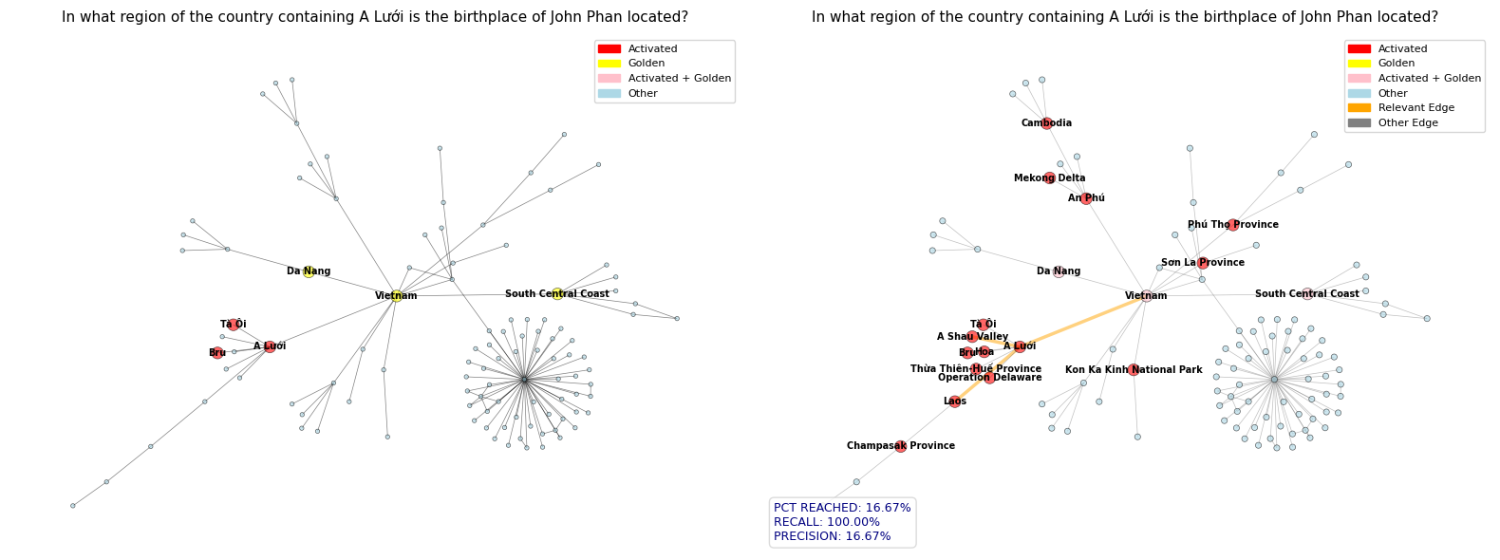
\includegraphics[width=\linewidth]{retrieval_ilustration.png}
  \caption{Spreading activation on the subgraph fetched for the query \textit{3hop2\_\_655849\_223623\_162182} from MuSiQue dataset. Golden entities are marked in yellow, activated entities in red, unactivated entities in light blue, and activated golden entities in pink.}
  \label{fig:fig4}
\end{figure}

After obtaining the set of activated entities, we fetch the set of documents $\mathcal{D} = \{D_{1},...D_{k_1}\}$  from the knowledge base, consisting of document nodes that have outgoing \textit{describes} links connecting them to the activated entity nodes. Here, we also perform filtering by removing documents whose cosine similarity to the query is lower than the pruning threshold  $\tau_{d}$. Additionally, we augment the set of retrieved documents with the textual representations of relevant relationships $r_1,... r_{k_2}$ between activated entities, as encoded in the links between them. A relationship is considered relevant if its weight, determined based on cosine similarity at the beginning, exceeds the threshold  $\tau_r$. In this way, we obtain the final context $\mathcal{C} = \{D_{1},...D_{k_1},r_1,... r_{k_2}\}$, which is then passed to the LLM in the next stage. We found that threshold values $\tau_a = 0.5$, $\tau_d = 0.45$, and $\tau_r = 0.5$ work well in practice.


\begin{figure}[ht]
  \centering
  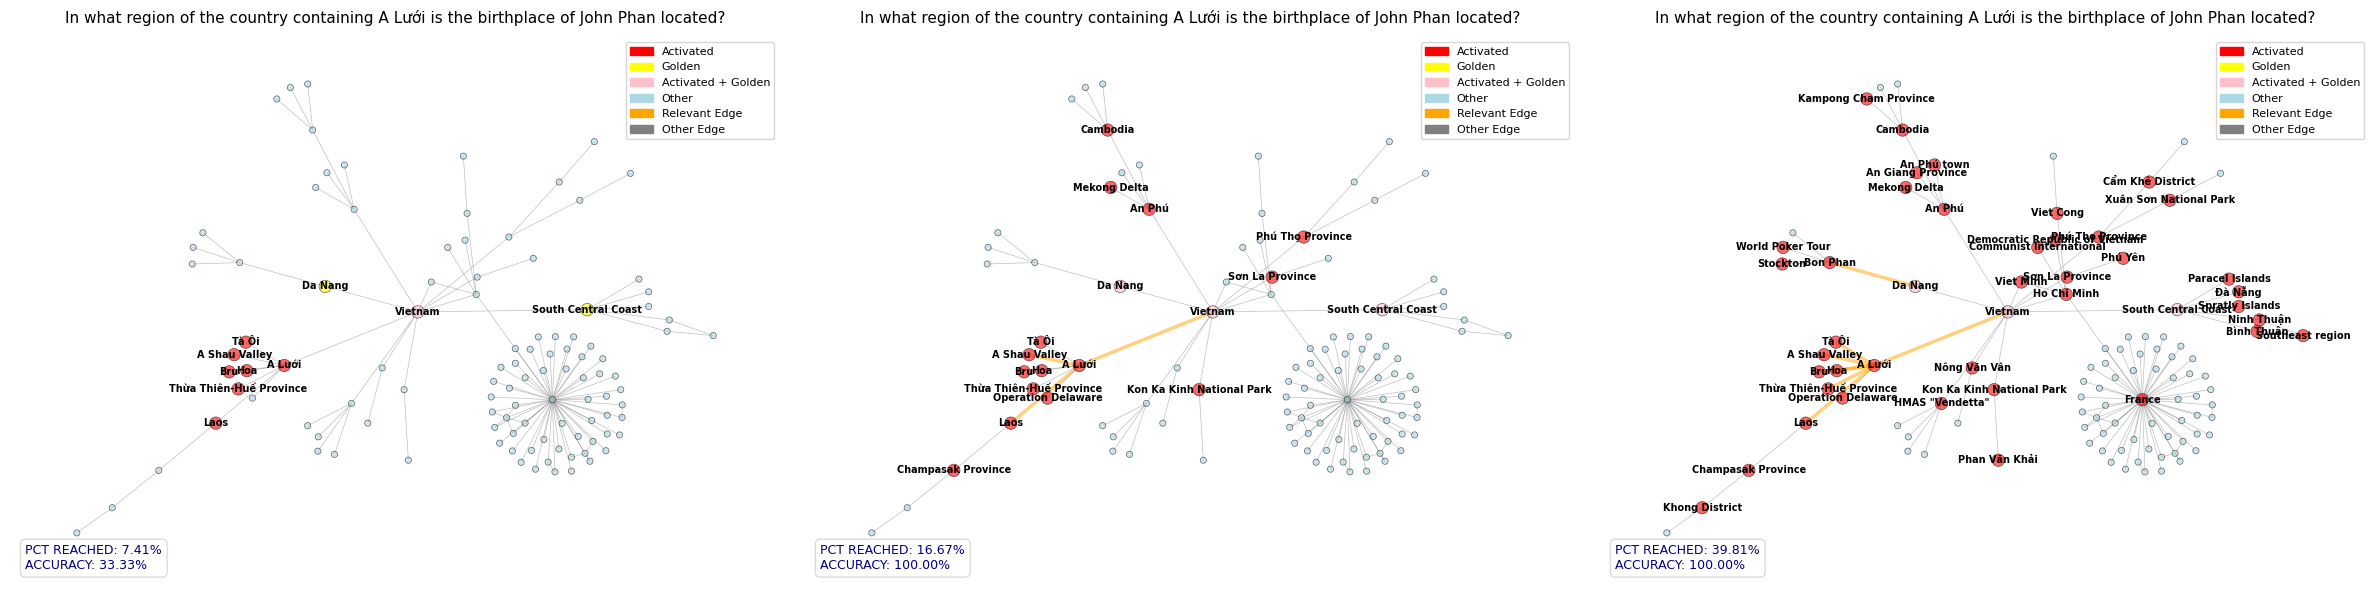
\includegraphics[width=\linewidth]{parameters_3hop2__655849_223623_162182.png}
  \caption{Effect of applying a linear normalization factor to the edge weights of the fetched subgraph on spreading activation dynamics. The first column corresponds to $c = 0.5$, the second to $c = 0.4$, and the third to $c = 0.3$.}
  \label{fig:fig5}
\end{figure}

\subsection{Answer generation}
Finally, provided with the fetched context and the multi-hop query, the LLM is instructed to reason through the knowledge text in a step-by-step manner, verifying all arithmetic calculations if the question requires quantitative reasoning. It then outputs its reasoning and the final answer if it is able to deduce one based solely on the provided knowledge, or otherwise notes that the question is not answerable based on the retrieved information.

\section{Experiment Design and Evaluations}
This section describes how the proposed method is evaluated and what it is compared against. It first introduces the benchmarks and the evaluation setup, and then we proceed by defining the baseline RAG and GraphRAG methods used for comparison, and clarifying the role of iterative variants. 

\subsection{Benchmarks}
We evaluate our system on two well-known MHQA benchmarks: MuSiQue~\cite{musique} and 2WikiMultiHopQA~\cite{2wiki}.

One of the earliest and most widely used multi-hop QA datasets was HotpotQA~\cite{hp}, created through crowdsourced multi-hop questions over Wikipedia articles. However, it has faced considerable criticism for not consistently requiring genuine multi-hop reasoning, as many questions could be answered through dataset artifacts or inference shortcuts~\cite{hp_criticism1, hp_criticism2, hp_criticsm3}.

In response, 2WikiMultiHopQA~\cite{2wiki} refined the evaluation paradigm by combining unstructured Wikipedia text with structured Wikidata knowledge, thereby mitigating some of these issues. MuSiQue~\cite{musique} advanced this approach further by composing multi-hop questions in a bottom-up manner from a large pool of single-hop questions while enforcing strict connected reasoning. Therefore, in our experiments, we used 2WikiMultiHopQA and MuSiQue to evaluate the performance gains introduced by our methodology. 

Given the high computational expense associated with LLM-based knowledge graph construction, we restrict our evaluation to a random subset of 100 questions per benchmark.

\subsection{Baselines}
In the experiments, we include four different types of baseline RAG methods against which we compare our proposed pipeline.

First, we employ the Naive RAG baseline, which retrieves the top-$k$ documents with the highest cosine similarity between their embeddings and the query embedding, and feeds them directly into the LLM’s prompt together with the input query. We evaluate two variants of this baseline, with $k = 5$ and $k = 10$.

Second, we consider CoT-based RAG systems, which perform iterative retrieval. Here, the LLM is prompted to reason over the context gathered in each retrieval step and attempt to answer the original question. If the answer cannot be determined from the current context, the LLM formulates a follow-up question, based on which a new context is fetched and added to a short-term memory containing summarised knowledge from previous steps. This process runs sequentially for a pre-specified maximum of three steps (as increasing the number of steps beyond this did not improve performance). We also have two variants for this method for top-$k$ values of 5 and 10.

Third, we have a system based on query-decomposition methodology, where the LLM is prompted to decompose a complex question into a sequence of simpler, preferably single-hop queries, which are then used to sequentially gather context and derive intermediate answers.

Finally, we use HippoRAG as a graph-based baseline, specifically the second version proposed in~\cite{gutierrez2025rag}, for which state-of-the-art performance is reported on the MHQA benchmarks used in our evaluation.

Details and exact prompts used for all baselines are provided in Appendix A.

\section{Results}
In this section, we evaluate SA-RAG on the previously described benchmarks and compare it against the baseline methods introduced in Section 3.2. We report Exact Match (EM) together with F1, an overlap-based metric that awards partial credit when the predicted answer shares content with the reference. Across all settings, a clear pattern emerges: SA-RAG is competitive as a standalone retriever, and it becomes most impactful when used within an iterative retrieval hook.

\begin{table}[h!]
    \centering
    \caption{Results of RAG evaluation on two multi-hop benchmarks.}
    \label{tab:rag_evaluation}

    %=================== Benchmark 2 ===================
    \begin{subtable}[t]{\textwidth}
        \centering
        \caption{MuSiQue}
        \label{tab:rag_bench2}
        \begin{tabular}{lcccccc}
            \toprule
            & \multicolumn{3}{c}{phi4} & \multicolumn{3}{c}{gemma3} \\
            \cmidrule(lr){2-4} \cmidrule(lr){5-7}
            Methodology & EM & F1 & Correctness & EM & F1 & Correctness \\
            \midrule
            Naive RAG            & 0.25 & 0.36 & 46 & 0.26 & 0.36 & 45 \\
            Naive RAG (k=10)     & 0.23 & 0.38 & 49 & 0.32 & 0.41 & 54 \\
            CoT RAG              & 0.33 & 0.44 & 56 & 0.39 & 0.50 & 58 \\
            CoT RAG (k=10)       & 0.33 & 0.46 & 56 & 0.34 & 0.45 & 56 \\
            Query-decomposition  & 0.34 & 0.48 & 56 & 0.40 & 0.51 & 61 \\
            HippoRAG 2           & 0.32 & 0.52 & 70 & 0.31 & 0.47 & 59\\
            SA-RAG               & 0.40 & 0.54 & 67 & 0.35 & 0.48 & 56 \\
            SA-RAG + CoT          & \textbf{0.44} & \textbf{0.61} & \textbf{75} & \textbf{0.43} & \textbf{0.57} & \textbf{69} \\
            SA-RAG + decomposition& 0.39 & 0.51 & 66 & 0.34 &  0.54 & 63 \\
            \bottomrule
        \end{tabular}
    \end{subtable}

    \vspace{0.5em}

    %=================== Benchmark 1 ===================
    \begin{subtable}[t]{\textwidth}
    \centering
    \caption{2WikiMultihopQA}
    \label{tab:rag_bench1}
    \begin{tabular}{lcccccc}
        \toprule
        & \multicolumn{3}{c}{phi4} & \multicolumn{3}{c}{gemma3} \\
        \cmidrule(lr){2-4} \cmidrule(lr){5-7}
        Methodology & EM & F1 & Correctness & EM & F1 & Correctness \\
        \midrule
        Naive RAG              & 0.36 & 0.42 & 48 & 0.36 & 0.44 & 48 \\
        Naive RAG (k=10)       & 0.46 & 0.52 & 58 & 0.49 & 0.57 & 62 \\
        CoT RAG                & 0.53 & 0.62 & 68 & 0.52 & 0.62 & 72 \\
        CoT RAG (k=10)         & 0.45 & 0.51 & 55 & 0.56 & 0.65 & 72 \\
        Query-decomposition    & 0.60 & 0.68 & 75 & 0.47 & 0.57 & 64 \\
        HippoRAG 2           & 0.50 & 0.62 & 76 & 0.58 & 0.69 & 75
        \\
        SA-RAG                 & 0.57 & 0.66 & 76 & 0.50 & 0.59 & 66 \\
        SA-RAG + CoT           & \textbf{0.72} & \textbf{0.78} & \textbf{87} & \textbf{0.58} & \textbf{0.69} & \textbf{77} \\
        SA-RAG + decomposition & 0.60 & 0.72 & 83 & 0.46 & 0.60 & 69 \\
        \bottomrule
    \end{tabular}
\end{subtable}

\end{table}

Table~\ref{tab:rag_evaluation} presents the experimental results, comparing the performance of different RAG approaches across the benchmarks. The experiments were conducted using two LLMs for reasoning and answer generation, \textit{phi4} and \textit{gemma3}, and \textit{BAAI/bge-large-en-v1.5} was used to generate the text embeddings. Beyond standard EM and F1 metrics, we included a manual \textit{Correctness} check to detect cases where the model produced semantically correct responses (e.g., valid aliases) that EM failed to reward, as well as for answers that obtained high F1 scores due to partial lexical overlap while remaining factually incorrect.

Two main observations can be drawn from the table. First, in experiments with the \textit{phi4} model, SA-RAG alone outperformed all iterative baselines on both benchmarks and achieved performance comparable to HippoRAG 2, with slightly lower correctness on MuSiQue. With \textit{gemma3}, however, HippoRAG 2 outperformed SA-RAG on both benchmarks, while the query-decomposition and CoT baselines outperformed it on MuSiQue. Our inspection of the retrieved context in the \textit{gemma3} experiments suggests that the absence of similar improvements was not due to missing or insufficient contextual information, but rather to limitations in the model’s reasoning. Although \textit{phi4} is smaller, it was specifically designed for complex reasoning tasks, unlike \textit{gemma3}. 

The second observation is that SA-RAG provides consistent performance gains when introduced as a plug-and-play module in any of the examined iterative pipelines, in all of the experiment setups. As shown in the table, combining SA-RAG with CoT retrieval yields the strongest performance, substantially outperforming all baseline RAG approaches, providing up to 10\% absolute gain in answer correctness over HippoRAG 2, and  25\% to 39\%  relative to Naive RAG.



\section{Conclusion \& Limitation}
In this paper, we addressed the challenges of document retrieval in RAG systems for complex tasks that require multi-step reasoning and evidence aggregation from multiple documents, such as MHQA. We proposed integrating the SA information retrieval algorithm with RAG approaches based on heterogeneous knowledge graphs to overcome the limitations of current systems without the need for expensive language model fine-tuning. Our experiments demonstrate the potential of this technique by achieving, with a single retrieval step, performance equivalent to or better than several advanced training-free baselines, and further show that it can be combined with methods like CoT to significantly boost system performance, even when using small open-weight language models.

However, several limitations of the current work should be acknowledged and addressed in future research. First, due to budget constraints and high experimental costs, we evaluated our method on a small sample of 100 randomly selected questions from each benchmark. More extensive validation is needed to empirically demonstrate the scalability of our system. Second, when assigning association weights to relationship links in the knowledge graph, we used cosine similarity values from an "off-the-shelf" embedding model and adapted them only through simple linear scaling for our task. Future work should explore improvements to the retrieval components, such as fine-tuning the embedding model for better task alignment.

\bibliographystyle{unsrt}  
\bibliography{references}  %%% Remove comment to use the external .bib file (using bibtex).
%%% and comment out the ``thebibliography'' section.


\appendix
\section{Implementation Details of Baseline RAG Methodologies}

In this appendix, we provide a detailed description of the implementation details for the baseline RAG methods evaluated in our experiments, including the retrieval systems and the prompts used. As specified, we consider three systems: \emph{Naive RAG}, \emph{CoT RAG} based on iterative retrieval, and a system based on \emph{query-decomposition prompting}. 

It is important to note that all three systems use the same prompt template, shown in Listing~\ref{lst:answering_bl}, to generate the final answer after the retrieval step. Once the relevant context is gathered from the document corpus, it is embedded into this template to instruct the LLM to reason over the retrieved information and produce a final answer in the form of a JSON object. This object uses the structured output capabilities of the LLM and contains two textual fields: \verb|reasoning| and \verb|final_answer|. Including the \verb|reasoning| field improves LLM performance by allowing the model to carry out intermediate deduction steps and calculations before producing the final answer, while also reducing the likelihood of unnecessary information appearing in the \verb|final_answer| field.


\begin{lstlisting}[style=baselinestyle, caption={Answering prompt for baseline systems}, label={lst:answering_bl}]
Below is a question followed by some context from different sources. Please answer the question based on the context. The answer to the question could be either single word, yes/no or consist of multiple words describing single entity. If the provided information is insufficient to answer the question, respond 'Insufficient Information'. Answer directly without explanation. Provide answer in JSON object with two string attributes, 'reasoning', which" provides your detailed reasoning about the answer, and 'final_answer' where you provide your short final answer without explaining your reasoning.
\end{lstlisting}

The design of the \emph{Naive RAG} system is relatively simple. First, the knowledge documents are split into overlapping chunks of 500 words, with an overlap size of 100 words, and stored in a database together with their vector embeddings. Given an input query, the embedding model generates a dense vector representation of the query text, which is then compared against the embeddings of the document chunks in the knowledge corpus to retrieve the \textit{top-$k$} most similar chunks based on cosine similarity.

\emph{CoT RAG}, on the other hand, performs a sequence of iterative retrieval steps. At each step, it determines whether the answer to the question can be inferred from the currently available information and generates a follow-up question if the answer cannot be deduced from the provided context. During each reasoning step, the LLM is also asked to summarize the information from the current context, and this summary is passed to subsequent steps to be combined with the text from newly retrieved chunks. The prompt used for this purpose is shown in Listing~\ref{lst:reasoning_bl}.

\begin{lstlisting}[style=baselinestyle, caption={Reasoning prompt for baseline systems}, label={lst:reasoning_bl}]
You are given a **multi-hop question** that requires combining information across multiple source documents. Along with the question, you are provided a list of **short knowledge paragraphs**, each with different pieces of information potentially required for answering the query.

## Task description

Your goal is to **understand and reason through the question** using only the information provided.

To achieve this you should:
- **Extract the relevant** facts from the knowledge paragraphs that are needed to answer the question.
- **Paraphrase and organize** these facts into a clear and coherent summary called 'provided_context'. This summary should explain how the relevant entities and relationships come together to support answering the question.
- Based on this reasoning:
    - If the information is **sufficient to directly answer the question**, provide the answer.
    - If important information is **missing**, return a **specific follow-up question** that would help fill the gap.

### Output Format (JSON)

```json
{
  "provided_context": "Summarize only the facts relevant to answering the question, combining them into a clear explanation.",
  "answer_possible": true | false,
  "final_answer": "Give your answer here if 'answer_possible' is true, otherwise leave this blank.",
  "additional_question": "If 'answer_possible' is false, write a clear and specific follow-up question that would help get the missing information."
}
```
# Input
You are given a **multi-hop question** that requires combining information across multiple source documents. Along with the question, you are provided: a list of **short knowledge paragraphs**, each describing specific entities and facts
```
# Input
\end{lstlisting}

Finally, Listing~\ref{lst:decompose} displays the prompt that serves as the backbone of the \emph{query-decomposition} method. Here, the LLM is asked to decompose a multi-hop query into a list of simpler queries whose answers provide intermediate steps needed to answer the original query. After decomposition, the system answers these simpler questions sequentially, one at a time, in the specified order.  At each step, the system first combines the current sub-query with the questions and answers from previous steps to generate a vector embedding for retrieval of the most relevant knowledge passages, and the LLM then uses this retrieved context to answer the current sub-query. Once all sub-queries have been answered, the system performs a final retrieval step based on an embedding of the original query to gather additional relevant documents. This retrieved context is then combined with the full list of sub-queries and their answers and provided to the LLM as context for deriving the final answer.


\begin{lstlisting}[style=baselinestyle, caption={Question decomposition prompt}, label={lst:decompose}]
You are a decomposition module for a multi-hop question answering system.
Your task: **given one user query, rewrite it as the smallest possible sequence of simpler, preferably single-hop questions** that, when answered in order, are sufficient to answer the original query.

Follow these rules strictly:

1. **Use only information explicitly present in the original query.**

   * Do **not** introduce new entities, definitions, or clarifying questions that the user did not ask.
   * If the query says “John Phan,” do **not** ask “Who is John Phan?” because that is not needed to resolve the chain.

2. **Decompose by inference steps, not by wording.**

   * Each subquestion should retrieve **one missing fact** or **resolve one reference** needed by a later subquestion.
   * Prefer single-hop, factual questions (entity → attribute, entity → location, entity → relation).

3. **Keep only necessary subquestions.**

   * If a fact is already given in the original query, do **not** restate it as a question.
   * Stop decomposing when the main query becomes answerable.

4. **Preserve dependency order.**

   * Later subquestions may refer to entities/answers from earlier ones.
   * Number the subquestions in the order they should be executed.

5. **Output format (JSON):**

   ```json
   {
     "original_question": "<the user question>",
     "subquestions": [
       {"id": 1, "question": "..."},
       {"id": 2, "question": "..."},
       {"id": 3, "question": "..."}
     ]
   }
   ```

6. **If the query is already single-hop, return it as one subquestion** in the same format.

**Worked example**

Input question:

> “The Argentine PGA Championship record holder has won how many tournaments worldwide?”

Decomposition:

```json
{
  "original_question": "The Argentine PGA Championship record holder has won how many tournaments worldwide?",
  "subquestions": [
    {
      "id": 1,
      "question": "Who is the record holder for the Argentine PGA Championship?"
    },
    {
      "id": 2,
      "question": "How many tournaments worldwide has that person won?"
    }
  ]
}
```

Notes:

* You **must not** create questions like “What is Argentine PGA Championship?” because they are not required to answer the original query.
* You **must not** guess missing constraints.
* Your objective is **faithful, minimal, query-conditioned decomposition**, not general elaboration.

# Input

\end{lstlisting}

\section{Prompts Used in the SA-RAG Framework}

Here, we list the exact language model prompts used at various stages of the proposed SA-RAG methodology. Listings~\ref{lst:ner} and \ref{lst:re} display the prompts employed in the indexing step for performing named entity recognition (NER) and relationship extraction (RE), respectively. Both prompts instruct the LLM to produce structured responses in the form of JSON objects and include one-shot demonstrations for the corresponding tasks.

When performing NER, the LLM is instructed to extract, in addition to entity names, the entity type, all name aliases, and entity descriptions (stored in the \textit{entity\_information} field). For each specific entity type, the LLM is instructed to identify certain types of descriptive information in order to avoid capturing duplicated information for multiple related entities. For example, for Geopolitical Entities (GPE) such as cities or countries, the LLM should avoid extracting context-dependent information and should focus only on general information (e.g., "South Africa is a country in southern Africa" and not "South Africa is the country where Elon Musk was born," since birthplace information is captured in the description of a person and via relationships). The extracted names and entity types are then used to create entity nodes in the knowledge graph. Extracted descriptions form entity description nodes, aliases support entity resolution, and identified relationships are used to create links connecting the nodes.

Listings~\ref{lst:reasoning_sa} and \ref{lst:answering_sa} present the reasoning and answering prompts, respectively. These prompts are similar to those used in \emph{CoT RAG}, but have been adapted to instruct the LLM to take into account retrieved information about the identified key relationships.

\begin{lstlisting}[style=promptstyle, caption={NER prompt},label={lst:ner}]
Given a textual paragraph, your task is to identify and extract entities from the provided text following the detailed step-by-step procedure described below:

- **Identify all entities explicitly mentioned in the text.**
   - Entities fall into one of four categories:
     - **PERSON**: Individual people.
     - **ORGANIZATION**: Companies, institutions, and organized groups.
     - **GPE** (Geopolitical Entities): Countries, cities, states, regions, or territories.
     - **MISC**: All other notable entities that don't fit the above categories, such as historical events, artworks, patents, buildings, etc.

- **Handle Names and Aliases:**
   - If an entity has multiple mentions (aliases or abbreviations), use the **full official name** as the primary reference.
   - Include all the mentioned aliases in output information

- **Extract factual attributes:**
   - For **PERSON** entities, extract:
     - Birthplace, birth/death dates, nationality, occupation, titles, and achievements explicitly stated in the text.
   - For **ORGANIZATION** entities, extract:
     - Foundation dates, location of headquarters, industry or sectors, associated institutions, co-founders, and explicit criticisms if any.
   - For **GPE** entities, extract:
     - Extract explicitly stated geographical or political details, historical characteristics, capital city, demographics, and cultural or administrative aspects
     - **By any means do not include** information like "birthplace of...", "city of origin of...", or "location where someone died" or any information that describe GPE in context dependent manner
   - For **MISC** entities, extract:
     - Explicitly stated temporal attributes, scale, historical significance, or explicit descriptive facts provided in the text.

- **Strict adherence to text:**
   - **Only** extract details explicitly mentioned in the text.
   - **Do not** infer, assume, or fabricate information not present in the provided text.

## Output Format

- Return your response as a JSON array.
- Each element in the array should be a JSON object with exactly four keys: `"name"`, `"type"`, `"aliases"`, and `"entity_information"`.

# Demonstration

## Input

Nikola Tesla (born July 9/10, 1856, Smiljan, Austrian Empire [now in Croatia]—died January 7, 1943, New York, New York, U.S.) was a Serbian American inventor and engineer who discovered and patented the rotating magnetic field, the basis of most alternating-current machinery. He also developed the three-phase system of electric power transmission. He immigrated to the United States in 1884 and sold the patent rights to his system of alternating-current dynamos, transformers, and motors to George Westinghouse. In 1891 he invented the Tesla coil, an induction coil widely used in radio technology.

## Desired output

[
  {
    "name": "Nikola Tesla",
    "type": "PERSON",
    "aliases": [],
    "entity_information": "Born July 9/10, 1856, in Smiljan, Austrian Empire (now in Croatia), died January 7, 1943, in New York, U.S. Serbian American inventor and engineer who discovered and patented the rotating magnetic field, developed the three-phase system of electric power transmission, immigrated to the United States in 1884, sold patent rights of alternating-current systems to George Westinghouse, and invented the Tesla coil in 1891."
  },
  {
    "name": "Smiljan",
    "type": "GPE",
    "aliases": [],
    "entity_information": "Place previously in Austrian Empire, currently part of Croatia."
  },
  {
    "name": "Austrian Empire",
    "type": "GPE",
    "aliases": [],
    "entity_information": "Empire existing in 1856."
  },
  {
    "name": "Croatia",
    "type": "GPE",
    "aliases": [],
    "entity_information": "Country in Europe."
  },
  {
    "name": "New York",
    "type": "GPE",
    "aliases": [],
    "entity_information": "City in the United States."
  },
  {
    "name": "United States",
    "type": "GPE",
    "aliases": ["U.S."],
    "entity_information": "Country."
  },
  {
    "name": "George Westinghouse",
    "type": "PERSON",
    "aliases": [],
    "entity_information": "Person who purchased patent rights of Nikola Tesla's system of alternating-current dynamos, transformers, and motors."
  },
  {
    "name": "Tesla coil",
    "type": "MISC",
    "aliases": [],
    "entity_information": "Induction coil invented by Nikola Tesla in 1891, widely used in radio technology."
  }
]

## Forbidden outputs

[
  {
    "name": "United States",
    "type": "GPE",
    "aliases": [],
    "entity_information": "Country where Nikola Tesla immigrated to in 1884."
  },
  {
    "name": "New York",
    "type": "GPE",
    "aliases": [],
    "entity_information": "City in the United States, where Nikola Tesla died."
  },
  {
    "name": "Smiljan",
    "type": "GPE",
    "aliases": [],
    "entity_information": "Town in the Austrian Empire (now in Croatia), birthplace of Nikola Tesla."
  }
]

# Real input    
\end{lstlisting}


\begin{lstlisting}[style=promptstyle, caption={RE prompt},label={lst:re}]
You are given a textual paragraph and a list of named entities. Your task is to perform relationship extraction by identifying all explicit relationships mentioned in the text that connect two entities from the provided list.

# Instructions:

- **Entity Pairing:** Only consider relationships between two entities from the provided named entities list.
- **Triple Format:** For each relationship found, output a triple formatted as a list of three strings: `["entity1", "relationship", "entity2"]`.
- **Pronoun Resolution:** Replace any pronouns with their corresponding specific named entities so that all references are clear.
- **Output Format:** Your final answer must be a JSON dictionary containing a single key `"triples"`, whose value is a list of all the extracted triples.
- **Explicit Relationships:** Only include relationships that are explicitly mentioned in the text.

# Demonstration

### Input
 
Jack Parsons (born October 2, 1914, Los Angeles, California, U.S.—died June 17, 1952, Pasadena, California) was an American rocket scientist and chemist who made significant contributions to the development of rocket technology and missile systems and was a cofounder of the Jet Propulsion Laboratory (JPL) at the California Institute of Technology (Caltech) and of the Aerojet Engineering Corporation.

Entity list: Jack Parsons, Los Angeles, Pasadena, Jet Propulsion Laboratory, California Institute of Technology, Aerojet Engineering Corporation

### Reasoning

1. **Identifing Provided Information:**  
   - **Input Text:** Reading the paragraph about Jack Parsons; Noting key phrases like "born in," "died in," "cofounder," and the association of JPL with Caltech.  
   - **Entity List:** Recognize the entities: Jack Parsons, Los Angeles, Pasadena, Jet Propulsion Laboratory, California Institute of Technology, Aerojet Engineering Corporation.

2. **Extracting Explicit Relationships:**  
   - Locating explicit statements in the text that connect two entities. For example, "Jack Parsons was born in Los Angeles" and "died in Pasadena."
   - Identifing that Jack Parsons "co-founded" both the Jet Propulsion Laboratory and the Aerojet Engineering Corporation.
   - Noting the phrase linking JPL to Caltech: "Jet Propulsion Laboratory at the California Institute of Technology."

3. **Performing Pronoun Resolution:**  
   - Ensuring that any pronouns referring to named entities are replaced by their proper names; In this case, no pronoun resolution was required since the entities are explicitly named.

### Response

{
  "triples": [
    ["Jack Parsons", "born in", "Los Angeles"],
    ["Jack Parsons", "died in", "Pasadena"],
    ["Jack Parsons", "co-founded", "Jet Propulsion Laboratory"],
    ["Jack Parsons", "co-founded", "Aerojet Engineering Corporation"],
    ["Jet Propulsion Laboratory", "is located at", "California Institute of Technology"]
  ]
}

# Real input
\end{lstlisting}


\begin{lstlisting}[style=promptstyle, caption={Answering prompt for SA-RAG},label={lst:answering_sa}]
You are given a multi-hop question and supporting context that describes relevant facts, entities and their relationships. Your task is to use the context to reason through the problem with clear, detailed, and correct step-by-step logic. Pay special attention to quantitative reasoning tasks; Verify every arithmetic calculation and check that the contextual details are interpreted accurately.
Proceed by first outlining all necessary steps to determine the answer, including any calculations or comparisons required. Once you have verified all arithmetic and double-checked key details, provide only a short final answer (which may be a single word, a yes/no, or a short phrase) without additional explanation.
Respond with a JSON object containing two string fields: 'reasoning', which provides your detailed reasoning about the answer, and 'final_answer' where you provide your short final answer without explaining your reasoning.
\end{lstlisting}


\begin{lstlisting}[style=promptstyle, caption={Reasoning prompt for SA-RAG},label={lst:reasoning_sa}]
You are given a **multi-hop question** that requires combining information across multiple textual paragraphs. Along with the question, you are provided:

1. **Short knowledge paragraphs**, each describing specific entities and facts.
2. A **list of key relationships** between these entities.

## Task description

Your goal is to **understand and reason through the question** using only the information provided.

To achieve this you should:
1. **Identify** only the facts and relationships that are directly relevant to answering the question.
2. **Paraphrase and weave** those facts into one concise, coherent paragraph called `provided_context`.
   - Write in full sentences.
   - Avoid listing facts one per line.
3. Decide whether you can answer the question with the information in your summary:
   - If **yes**, set `"answer_possible": true` and put your answer in `final_answer`.
   - If **no**, set `"answer_possible": false` and craft a specific follow-up question in `additional_question` that would help fill the gap in provided information

### Output Format (JSON)

```json
{
  "provided_context": "A single narrative paragraph summarizing all relevant facts.",
  "answer_possible": true | false,
  "final_answer": "Give your answer here if 'answer_possible' is true, otherwise leave this blank.",
  "additional_question": "If 'answer_possible' is false, write a clear and specific follow-up question that would help get the missing information."
}
```
# Input
\end{lstlisting}




\end{document}
